% !TEX program = xelatex
\documentclass[11pt,a4paper]{article}
\usepackage[margin=2cm]{geometry}
\usepackage{fontspec}
\setmainfont{DejaVu Serif}
\setsansfont{DejaVu Sans}
\usepackage{polyglossia}
\setdefaultlanguage{vietnamese}
\usepackage{amsmath,booktabs,array,graphicx,float,multirow,xcolor,hyperref,caption}
\usepackage{enumitem}
\usepackage{titlesec}
\usepackage{fancyhdr}
\usepackage{tikz}
\definecolor{ptitblue}{HTML}{0B3D91}
\definecolor{ptitred}{HTML}{C8102E}
\hypersetup{colorlinks=true,linkcolor=ptitblue,urlcolor=ptitblue,pdftitle={Phân tích và dự đoán giá bất động sản tại Hà Nội}}
\titleformat{\section}{\large\bfseries\color{ptitblue}}{\thesection.}{0.45em}{}
\pagestyle{fancy}\fancyhf{}
\fancyhead[L]{\small Phân tích và dự đoán giá bất động sản Hà Nội}
\fancyhead[R]{\small Nhóm 01 - Lập trình Python}
\cfoot{\thepage}\renewcommand{\headrulewidth}{0.4pt}
\setlength{\parindent}{0pt}\setlength{\parskip}{4pt}
\setlength{\emergencystretch}{3em}
\sloppy
\renewcommand{\arraystretch}{1.15}
\newcommand{\fig}[2]{\begin{figure}[H]\centering\includegraphics[width=#1\linewidth]{figures/#2}\end{figure}}
\begin{document}

% PAGE 1
\begin{titlepage}
\begin{tikzpicture}[remember picture,overlay]
  \draw[line width=1.5pt,ptitblue] ([xshift=1.1cm,yshift=-1.1cm]current page.north west) rectangle ([xshift=-1.1cm,yshift=1.1cm]current page.south east);
  \draw[line width=.6pt,ptitblue] ([xshift=1.25cm,yshift=-1.25cm]current page.north west) rectangle ([xshift=-1.25cm,yshift=1.25cm]current page.south east);
  \foreach \x/\y in {1.25/-1.25,-1.25/-1.25,-1.25/1.25,1.25/1.25}{\fill[ptitblue] ([xshift=\x cm,yshift=\y cm]current page.north west) circle (2pt);}
\end{tikzpicture}
\centering
\vspace*{1.15cm}
\begin{minipage}{\textwidth}\centering
{\Large\bfseries HỌC VIỆN CÔNG NGHỆ}\\[-.12cm]
{\Large\bfseries BƯU CHÍNH VIỄN THÔNG}\\[.3cm]
{\large KHOA TÀI CHÍNH KẾ TOÁN 1}\\[.65cm]

\includegraphics[width=.15\textwidth]{ptit-logo.jpg}\\[.55cm]
{\color{ptitblue}\rule{.86\textwidth}{1.4pt}}\\[.25cm]
{\LARGE\bfseries PHÂN TÍCH VÀ DỰ ĐOÁN GIÁ\\BẤT ĐỘNG SẢN TẠI HÀ NỘI\\KẾT HỢP MACHINE LEARNING}\\[.3cm]
{\color{ptitblue}\rule{.86\textwidth}{1.4pt}}
\end{minipage}\\[.65cm]
\vfill
{\Large Báo cáo bài tập lớn Python}\\[.45cm]
\begin{tabular}{rl}
\textbf{Nhóm:} & Nhóm 01 - Lập trình Python\\
\textbf{Thành viên:} & \begin{tabular}[t]{@{}l@{\hspace{1.2em}}l@{}}Tô Thành Công & B25DCTC024\\Bùi Quốc Anh & B25DCTC004\\Đặng Đức Anh & B25DCTC013\\Trần Hoàng Dũng & B25DCTC030\\Dương Minh Tuấn & B25DCTC132\end{tabular}\\
\textbf{GVHD:} & Lương Ngọc Sơn\\
\end{tabular}
\vfill {\large Hà Nội, 2026}
\end{titlepage}

% PAGE 2
\section{Tóm tắt và mục tiêu}
Nghiên cứu xây dựng pipeline phân tích dữ liệu và dự đoán giá rao bán bất động sản tại Hà Nội. Dữ liệu được làm sạch, loại trùng, phân tích theo nhiều chiều và đưa vào các mô hình hồi quy. Mục tiêu chính là so sánh mô hình trên thiết kế kiểm thử hạn chế rò rỉ, sau đó giải thích các yếu tố ảnh hưởng đến dự báo.

Kết quả tốt nhất thuộc về LightGBM tuning. Trên Group Split, mô hình đạt $R^2=0{,}800$, MAE $4.010{,}9$ triệu VNĐ, RMSE $11.678{,}6$ triệu VNĐ và MedAE $1.346{,}4$ triệu VNĐ. Đánh giá theo thời gian vẫn đạt $R^2=0{,}790$, cho thấy kết quả ổn định tương đối khi chuyển từ dữ liệu năm 2025 sang năm 2026.

\section{Dữ liệu và làm sạch}
Nguồn dữ liệu là bộ \texttt{locngodev/vietnam-real-estate} trên Kaggle, gồm các tin rao bán với 19 cột. Báo cáo sử dụng giá rao bán, không diễn giải thành giá giao dịch đã chốt.

\begin{table}[H]\centering\small
\caption{Quy mô dữ liệu qua các bước xử lý}\begin{tabular}{lrr}\toprule
Bước & Số dòng & Tỷ lệ giữ\\\midrule
Dữ liệu thô toàn quốc & 3.500.744 & 100,00\%\\
Lọc Hà Nội & 1.140.542 & 32,58\%\\
Giá và diện tích dương & 1.035.822 & 90,82\%\\
Loại trùng nghiệp vụ & 783.600 & 75,65\%\\
Tập dùng fit mô hình & 780.353 & 99,59\%\\\bottomrule
\end{tabular}\end{table}

Tập 783.600 dòng được giữ cho mô tả thị trường. Bộ lọc cực đoan chỉ áp dụng cho population dùng huấn luyện, tránh thay đổi bằng chứng EDA. Median được ưu tiên trong thống kê mô tả do phân phối giá lệch phải mạnh.

\section{Câu hỏi phân tích}
\begin{enumerate}[leftmargin=1.4em,itemsep=1pt,topsep=2pt]
\item Dữ liệu thiếu tập trung ở những trường nào và khác biệt ra sao giữa các loại hình?
\item Giá rao bán, diện tích và đơn giá/m$^2$ lệch phải và có ngoại lệ ở mức nào?
\item Nguồn cung, giá trung vị và đơn giá/m$^2$ chênh lệch ra sao giữa 5 phân khúc?
\item Mật độ tin và mặt bằng giá phân hóa thế nào giữa nội thành và ngoại thành?
\item Diện tích, số phòng, mặt tiền tương quan ra sao với giá và đơn giá?
\item Mô hình cây cải thiện bao nhiêu so với baseline và Ridge; sai số theo phân khúc thế nào?
\item Kết quả có ổn định khi dự báo 2026 từ dữ liệu 2025, và đặc trưng nào chi phối nhất theo Tree SHAP?
\end{enumerate}
\newpage

% PAGE 3
\section{Phân tích khám phá dữ liệu}
Giá và diện tích có độ lệch phải rõ rệt. Vì vậy, nhóm sử dụng cả thang đo gốc để diễn giải đơn vị tiền và thang log để quan sát phần lớn quan sát. Giá trung vị của tập sạch là 9.500 triệu VNĐ; đơn giá trung vị là 183,5 triệu VNĐ/m$^2$.

\begin{figure}[H]\centering
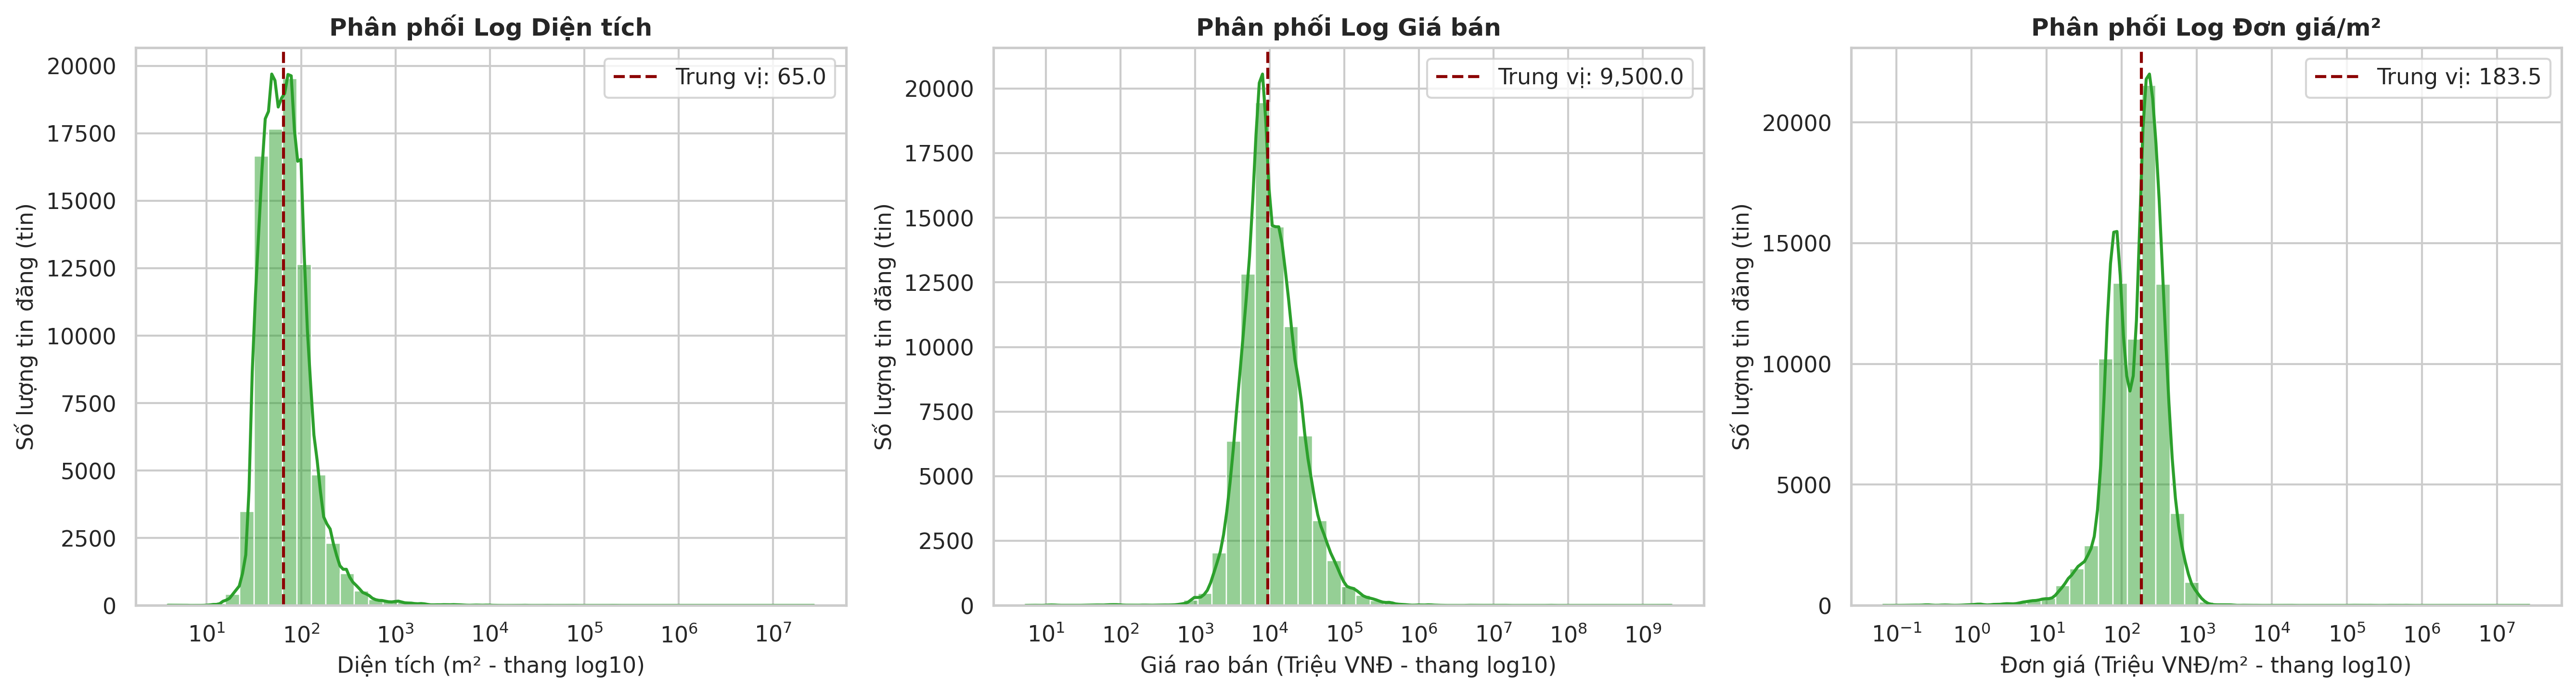
\includegraphics[width=.78\linewidth]{figures/E02_log_scale.png}
\caption{Phân phối diện tích, giá rao bán và đơn giá trên thang log10.}\end{figure}

\begin{figure}[H]\centering
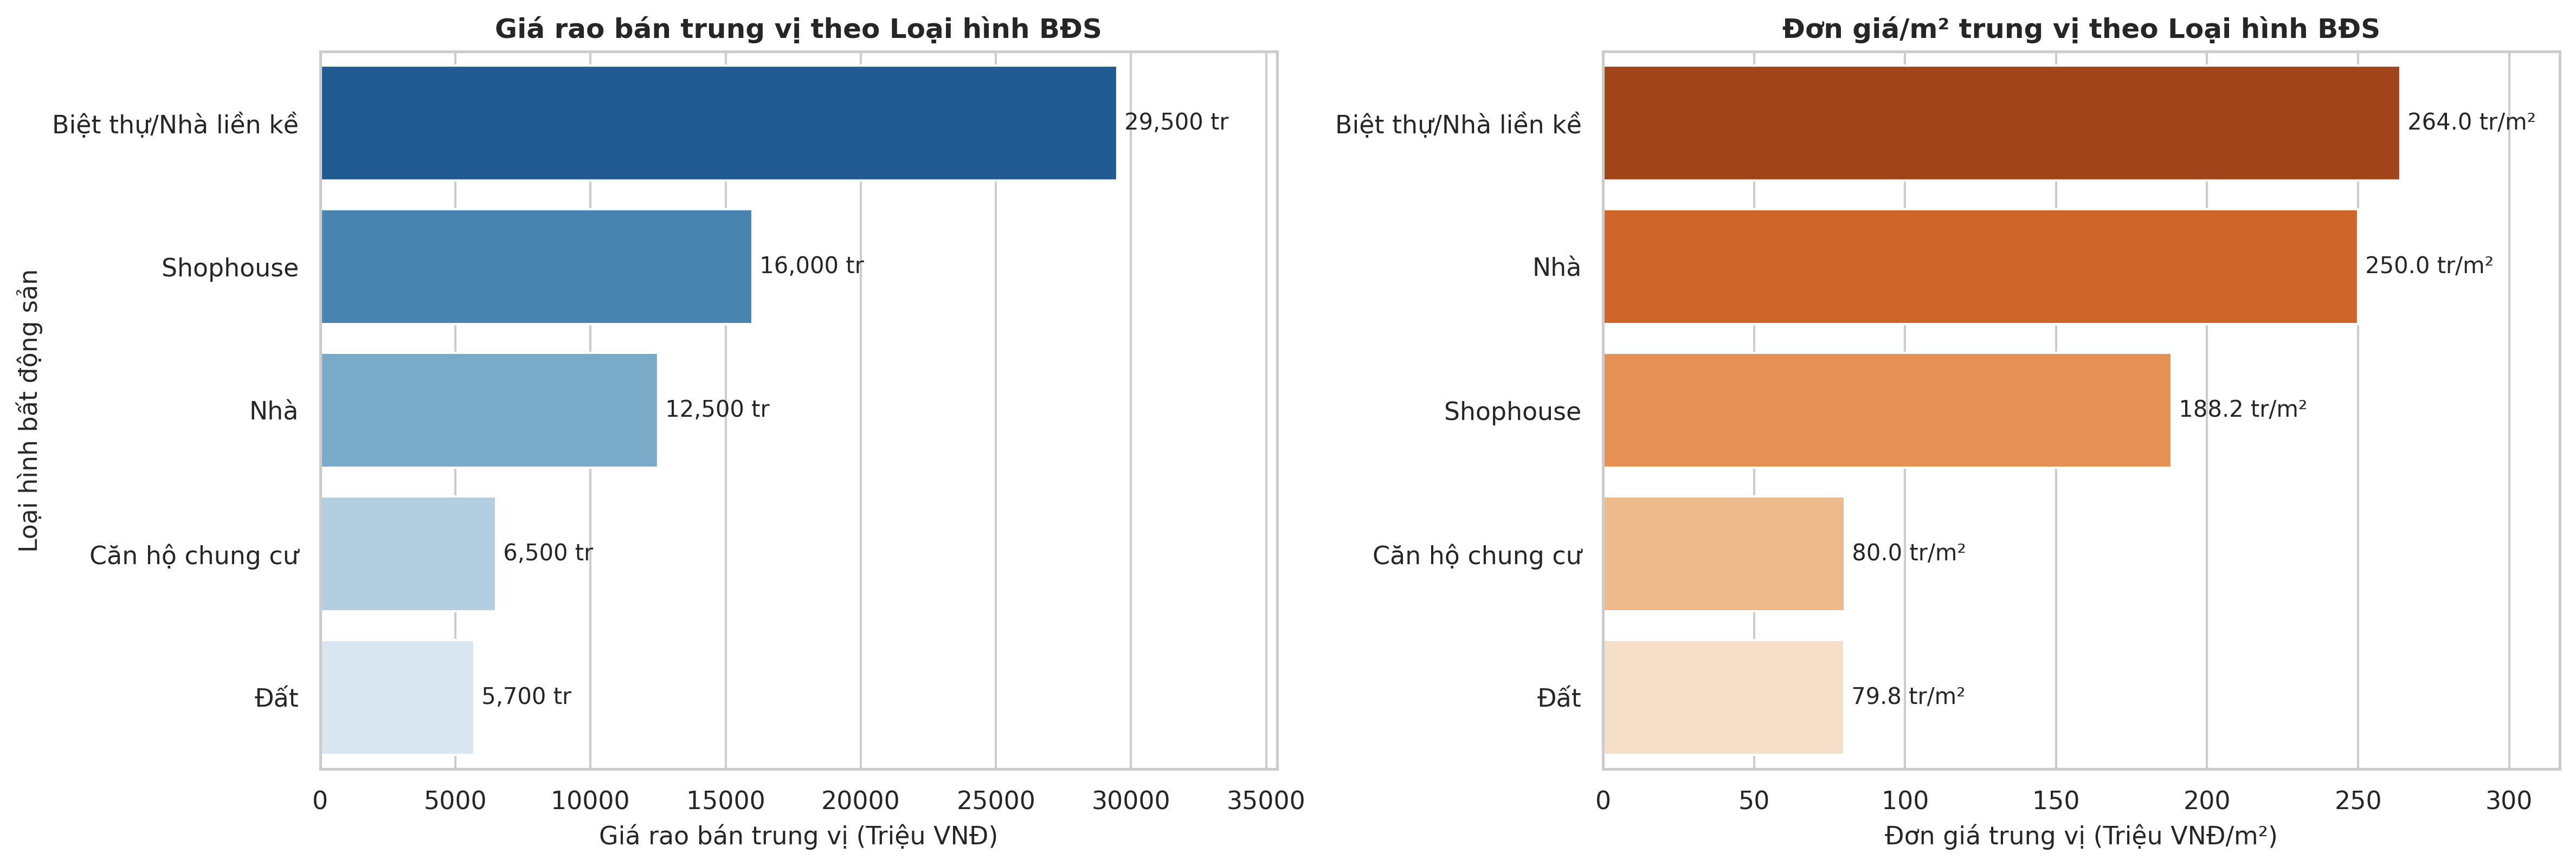
\includegraphics[width=.78\linewidth]{figures/E03_property_type_medians.png}
\caption{Giá trung vị theo nhóm loại hình bất động sản.}\end{figure}

So sánh theo loại hình cho thấy căn hộ có mức giá và độ phân tán thấp hơn tương đối, trong khi đất và shophouse có độ phân tán lớn hơn. Đây là lý do \texttt{property\_type\_name} được giữ trong pipeline mô hình.
\newpage

% PAGE 4
\section{Phương pháp}
\subsection{Đặc trưng và target}
Các biến số gồm diện tích, số tầng, mặt tiền, chiều sâu, chiều rộng đường, số phòng ngủ, số phòng tắm, năm và tháng đăng tin. Các biến phân loại gồm loại hình, quận/huyện, phường/xã, đường, hướng nhà và hướng ban công. \texttt{name} và \texttt{description} không đưa trực tiếp vào mô hình vì có thể chứa giá; \texttt{name} chỉ dùng tạo group key.

Mô hình học trên $y=\log(1+price)$ và chuyển ngược bằng $\operatorname{expm1}$. LightGBM dùng objective \texttt{regression\_l1}. Các biến phân loại hiếm được gộp vào \texttt{\_\_OTHER\_\_}; giá trị thiếu được xử lý theo khả năng của mô hình cây.

\subsection{Thiết kế kiểm thử}
Group key ưu tiên \texttt{project\_name}; nếu thiếu thì dùng \texttt{name} chuẩn hóa. Chia dữ liệu bằng \texttt{GroupShuffleSplit(n\_splits=1, test\_size=0.2, random\_state=42)}. Không có group giao nhau giữa train và test. Tuning thực hiện trên train, test chỉ dùng ở đánh giá cuối.

Để kiểm tra tính ổn định theo thời gian, nhóm dùng Time Split: train gồm tin năm 2025 và test gồm tin năm 2026. Đây là kiểm tra bổ sung, không thay thế Group Split.

\subsection{Mô hình so sánh}
Nhóm so sánh baseline median theo loại hình, Ridge Regression, Random Forest, HistGradientBoosting, XGBoost và LightGBM. Chỉ tiêu báo cáo gồm MAE, RMSE, MedAE, $R^2$ và MAPE trên giá gốc.
\newpage

% PAGE 5
\section{Kết quả mô hình}
\begin{table}[H]\centering\scriptsize
\caption{So sánh mô hình trên Group Split}\begin{tabular}{lrrrrr}\toprule
Mô hình & \shortstack{MAE\\{\scriptsize(triệu VNĐ)}} & \shortstack{RMSE\\{\scriptsize(triệu VNĐ)}} & \shortstack{MedAE\\{\scriptsize(triệu VNĐ)}} & $R^2$ & \shortstack{MAPE\\{\scriptsize(\%)}}\\\midrule
\textbf{LightGBM} & \textbf{4.011} & \textbf{11.679} & \textbf{1.346} & \textbf{0,800} & \textbf{22,5\%}\\
HistGradientBoosting & 4.171 & 12.217 & 1.397 & 0,781 & 23,2\%\\
XGBoost & 4.199 & 12.150 & 1.468 & 0,783 & 23,2\%\\
Random Forest & 4.883 & 14.773 & 1.651 & 0,680 & 26,9\%\\
Ridge Regression & 6.857 & 22.315 & 2.489 & 0,269 & 38,5\%\\
Baseline median & 9.563 & 25.466 & 4.000 & 0,048 & 55,9\%\\\bottomrule
\end{tabular}\end{table}

\begin{figure}[H]\centering
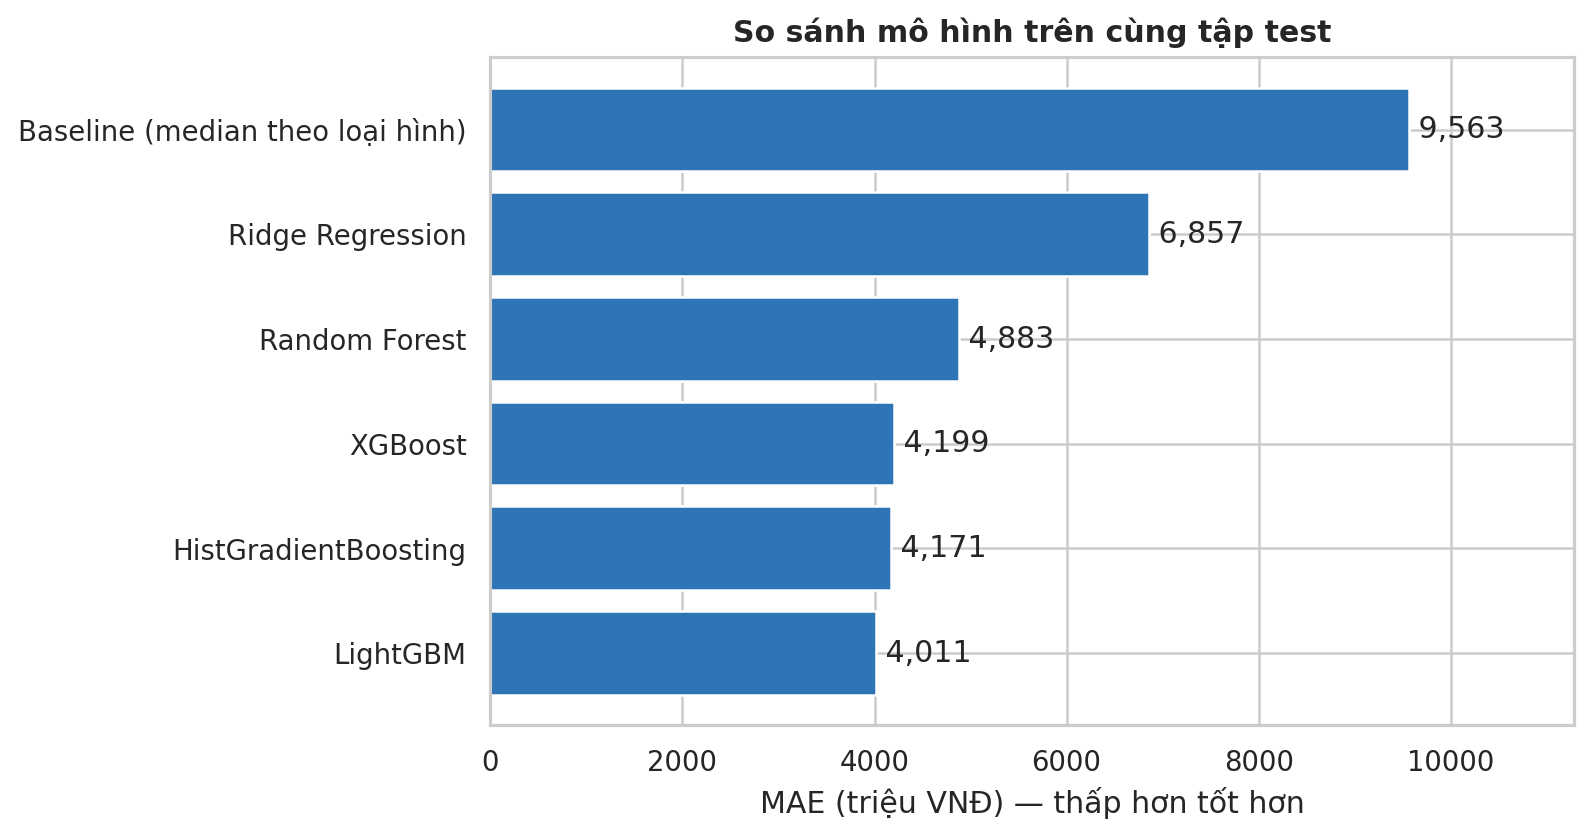
\includegraphics[width=.82\linewidth]{figures/02_model_comparison.png}
\caption{So sánh MAE giữa các mô hình trên Group Split (triệu VNĐ).}\end{figure}

LightGBM có MAE, RMSE và MedAE thấp nhất, đồng thời $R^2$ cao nhất. Chênh lệch giữa LightGBM và baseline cho thấy các đặc trưng về diện tích, loại hình và vị trí mang thông tin dự báo đáng kể. Tuy nhiên, RMSE lớn hơn MAE nhiều lần, phản ánh ảnh hưởng của một số tin có giá trị rất lớn hoặc đặc trưng thiếu.
\newpage

% PAGE 6
\section{Phân tích sai số và khả năng giải thích}
\subsection{Sai số theo thời gian}
Time Split cho kết quả: train năm 2025 có 630.403 dòng, test năm 2026 có 149.950 dòng; MAE 4.769 triệu VNĐ, RMSE 13.556 triệu VNĐ, MedAE 1.705 triệu VNĐ, $R^2=0{,}790$ và MAPE 23,5\%. Kết quả thấp hơn nhẹ so với Group Split, phù hợp với khó khăn khi dự báo giai đoạn mới.

\begin{figure}[H]\centering
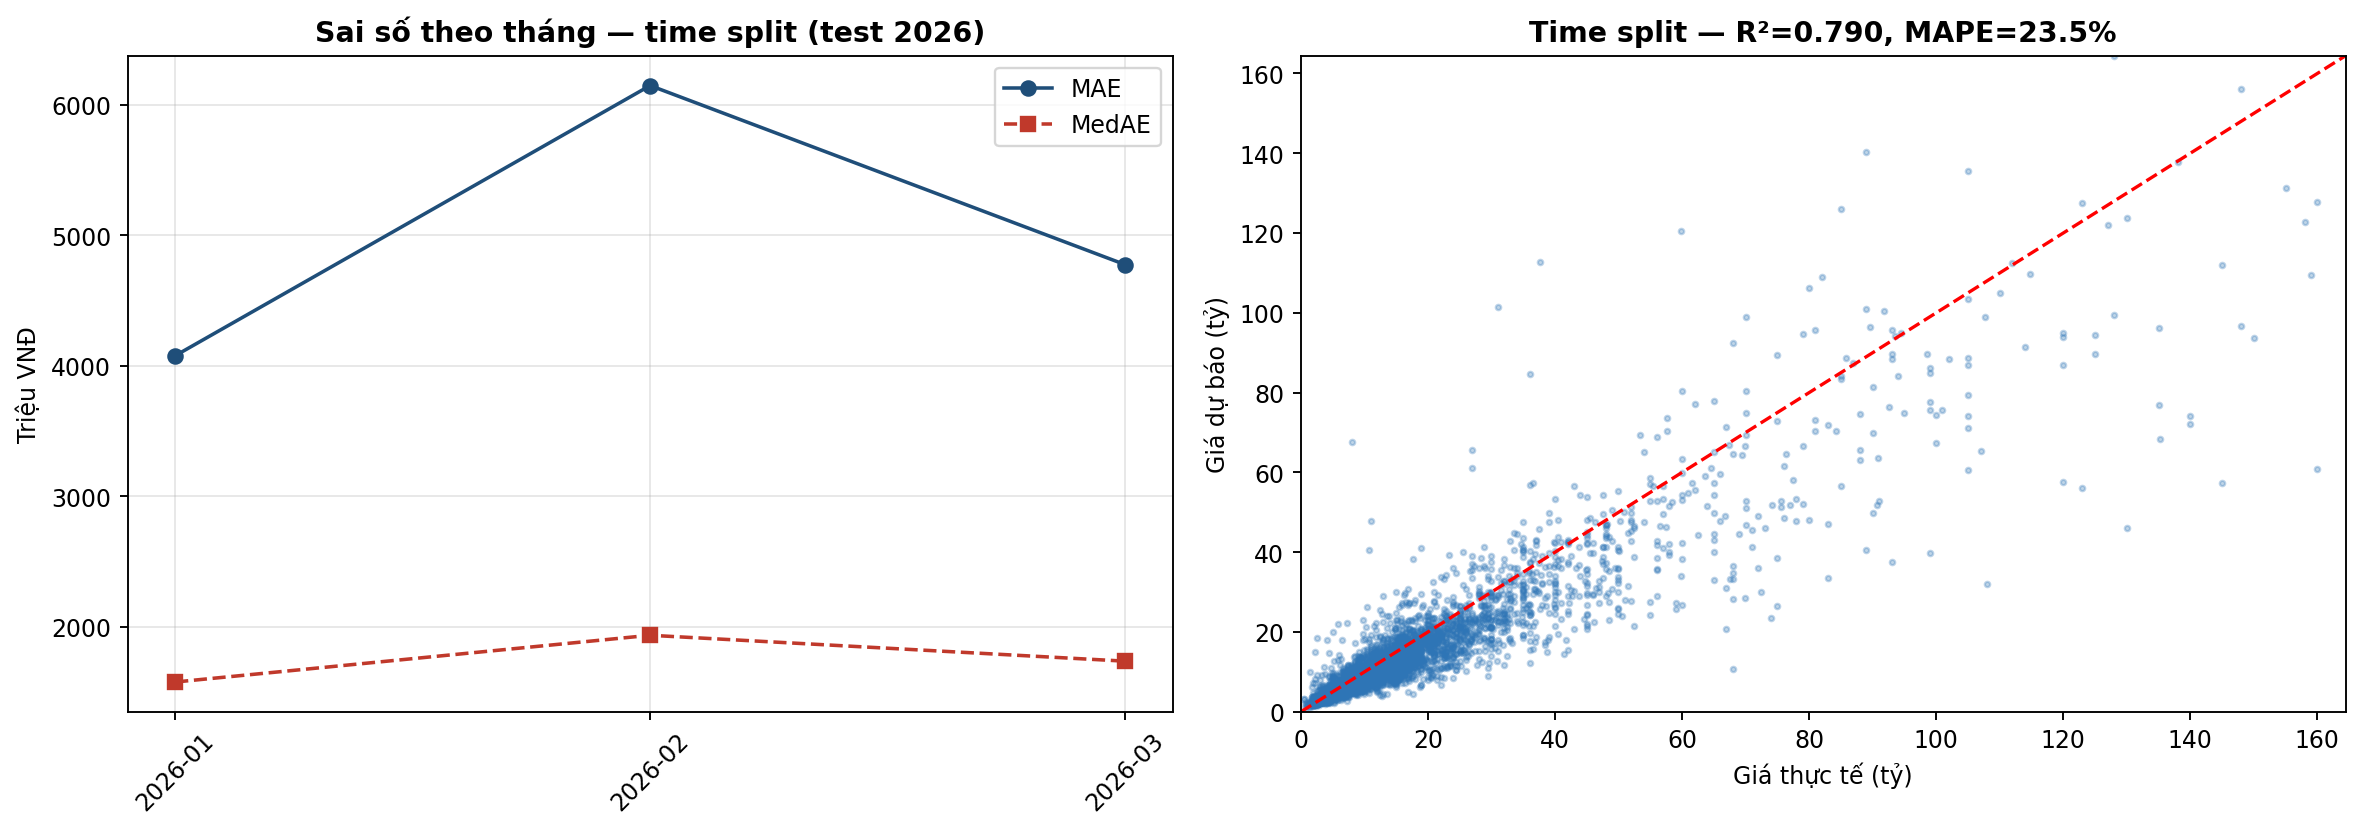
\includegraphics[width=.78\linewidth]{figures/05_time_split.png}
\caption{So sánh MAE giữa Group Split và Time Split (triệu VNĐ).}\end{figure}

\subsection{Sai số theo phân khúc}
Căn hộ có MAE 1.448 triệu VNĐ và $R^2=0{,}696$; nhà có MAE 4.584 triệu VNĐ và $R^2=0{,}820$; đất có MAE 3.073 triệu VNĐ và $R^2=0{,}810$; shophouse có MAE 12.273 triệu VNĐ và $R^2=0{,}342$. Shophouse có ít quan sát và tính dị biệt cao nên khó dự báo hơn.

\subsection{Đặc trưng quan trọng}
Theo Tree SHAP, \texttt{area} chiếm 30,6\%, \texttt{property\_type\_name} 27,3\%, \texttt{district\_name} 16,0\% và \texttt{ward\_name} 6,6\%. Bốn nhóm đầu chiếm 80,5\% tổng ảnh hưởng. Đây là diễn giải tương quan dự báo, không phải kết luận nhân quả.
\newpage

% PAGE 7
\section{Kết luận và giới hạn}
Nghiên cứu đã hoàn thành pipeline từ làm sạch dữ liệu đến đánh giá mô hình với tập 783.600 tin rao bán Hà Nội. Group Split và Time Split được dùng song song để giảm rủi ro đánh giá lạc quan. LightGBM tuned là mô hình phù hợp nhất trong các mô hình thử nghiệm, nhưng kết quả cần được hiểu là ước lượng giá rao bán.

Ba kết luận chính: (1) diện tích, loại hình và vị trí là nhóm thông tin quan trọng nhất; (2) mô hình cây tăng cường vượt baseline và Ridge trên cùng tập test; (3) sai số tăng mạnh ở nhóm shophouse và các tin có giá trị cực lớn.

\subsection{Giới hạn}
Dữ liệu không có ID bất động sản chắc chắn, nên group key từ dự án hoặc tiêu đề chỉ là proxy. Giá trong tin có thể không phản ánh giá giao dịch cuối cùng. Các yếu tố pháp lý, chất lượng nội thất, hướng view và tình trạng công trình chưa được mô tả đầy đủ. Time Split chỉ kiểm tra giai đoạn 2026 có trong dữ liệu, chưa đại diện cho cả năm.

\subsection{Tái lập}
Không đưa file dữ liệu 3,2 GB vào gói nộp. Người dùng có thể chạy notebook trên Kaggle bằng cách gắn dataset \texttt{locngodev/vietnam-real-estate} qua **Add Input**. Mã nguồn, notebook, bảng kết quả, \texttt{requirements.txt}, bảng phân công và báo cáo được đóng gói riêng. Các bước chạy được mô tả trong README.

\subsection{Tài liệu tham khảo}
\begin{enumerate}[leftmargin=1.5em,itemsep=1pt]
\item Kaggle, ``Vietnam Real Estate'', dataset ref: \texttt{locngodev/vietnam-real-estate}.
\item Pedregosa et al., ``Scikit-learn: Machine Learning in Python'', JMLR, 2011.
\item Ke et al., ``LightGBM: A Highly Efficient Gradient Boosting Decision Tree'', NeurIPS, 2017.
\item Lundberg \& Lee, ``A Unified Approach to Interpreting Model Predictions'', NeurIPS, 2017.
\end{enumerate}

\vfill\begin{center}\textit{Nhóm 01 - Lập trình Python · Hà Nội, 2026}\end{center}
\end{document}
